\begin{abstract}
  \setlength{\parskip}{1.5em}
  Surface-Enhanced Raman Spectroscopy can be used to study properties of graphene
  suspended on nanostructures. There is a common need to convert the local
  electromagnetic field amplitude enhancement that can be simulated to the total
  enhancement that usually is observed during an experiment.

  In this work there is a method presented to do this conversion using Lumerical~FDTD
  to simulate an experiment from ref.~\cite{heeg} and then using 3D modelling software
  to simulate and sculpt the graphene layer within the experiment. Both sets of data
  are combined to calculate the local and total enhancement of the surface-enhanced
  Raman scattering in the experiment.

  It will be shown that the projected electromagnetic field in the layer of graphene
  closely resemble the results of just using a planar slice at a height of \SI{40}{nm}
  and therefore confirm the approximations used in ref.~\cite{heeg}. Taking laser
  geometry and spatial coherence in near-field Raman scattering into account, a
  total enhancement of $23.0$ is calculated which was measured as $12.8$ by ref.~\cite{heeg}.

  The presented method is exemplarily executed with the above-mentioned experiment
  but can be adapted for any Raman-active material suspended on nanostructures for
  surface-enhanced Raman spectroscopy.

  \begin{figure*}[!h]
    \centering
    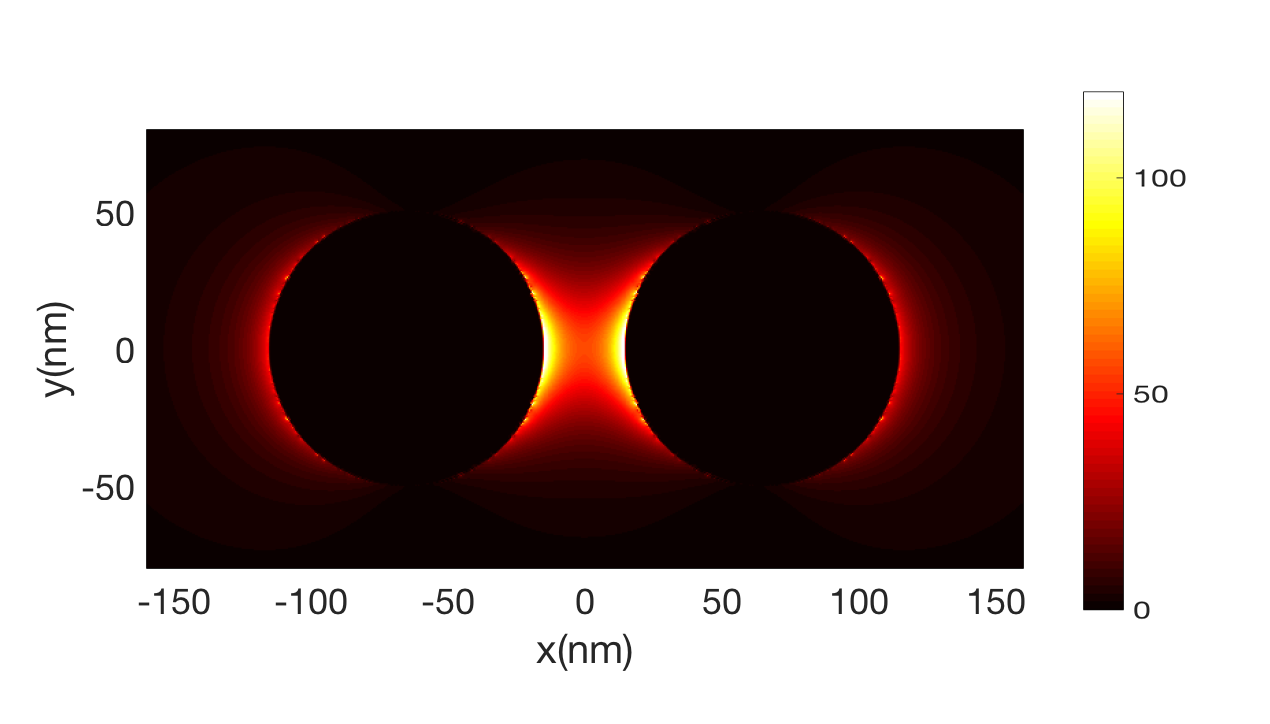
\includegraphics[width=0.7\textwidth]{./images/40nm.png}
  \end{figure*}
\end{abstract}
